\documentclass[12pt]{article}

\usepackage[english]{babel}
\usepackage[utf8]{inputenc}
\usepackage[top=2cm, left=2cm, right=2cm, bottom=2cm]{geometry}
\usepackage[document]{ragged2e}
\usepackage{tikz,minted,times}

\setlength\parindent{0pt}
\sloppy
\usetikzlibrary{automata,positioning,arrows,fit}
\tikzset{node distance=2.5cm,every state/.style={semithick,fill=gray!10},initial text={},double distance=2pt,every edge/.style={draw,->,>=stealth,auto,semithick}}
\usemintedstyle{colorful}

\title{COMP SCI 7411 Event Driven Computing Practice 2 Plan}
\author{Tinson Lai \\ a1812422}
\date{}

\begin{document}

\maketitle

\section{$\epsilon$-NFA}

The complete $\epsilon$-NFA for RegEx \mintinline{js}{/ba+a|(bc)+/} is

\begin{figure}[H]
  \centering

  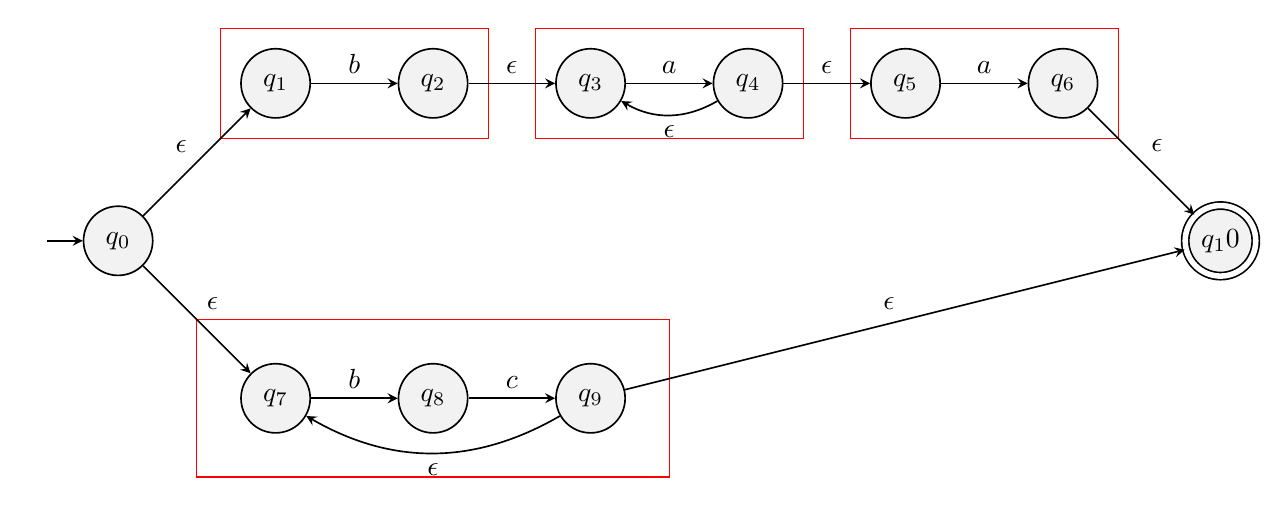
\begin{tikzpicture}
    \node[state, initial] at (0, 2) (q0){$q_0$};
    \node[state] at (2, 4) (q1){$q_1$};
    \node[state] at (4, 4) (q2){$q_2$};
    \node[state] at (6, 4) (q3){$q_3$};
    \node[state] at (8, 4) (q4){$q_4$};
    \node[state] at (10, 4) (q5){$q_5$};
    \node[state] at (12, 4) (q6){$q_6$};
    \node[state] at (2, 0) (q7){$q_7$};
    \node[state] at (4, 0) (q8){$q_8$};
    \node[state] at (6, 0) (q9){$q_9$};
    \node[state, accepting] at (14, 2) (q10){$q_10$};

    \node[draw = red, fit = (q1) (q2), inner sep = 0.25cm] {};
    \node[draw = red, fit = (q3) (q4), inner sep = 0.25cm] {};
    \node[draw = red, fit = (q5) (q6), inner sep = 0.25cm] {};
    \node[draw = red, fit = (q7) (q8) (q9), inner sep = 0.55cm] {};

    \draw

    (q0) edge node{$\epsilon$} (q1)
    (q0) edge node{$\epsilon$} (q7)

    (q1) edge node{$b$} (q2)
    (q2) edge node{$\epsilon$} (q3)
    (q3) edge node{$a$} (q4)
    (q4) edge[bend left] node{$\epsilon$} (q3)
    (q4) edge node{$\epsilon$} (q5)
    (q5) edge node{$a$} (q6)
    (q6) edge node{$\epsilon$} (q10)

    (q7) edge node{$b$} (q8)
    (q8) edge node{$c$} (q9)
    (q9) edge[bend left] node{$\epsilon$} (q7)
    (q9) edge node{$\epsilon$} (q10)

    ;
  \end{tikzpicture}

  \caption{$\epsilon$-NFA}
\end{figure}

which contains several unnecessary $\epsilon$-transitions representing concatenation. By removing those $\epsilon$-transitions, the $\epsilon$ becomes

\begin{figure}[H]
  \centering

  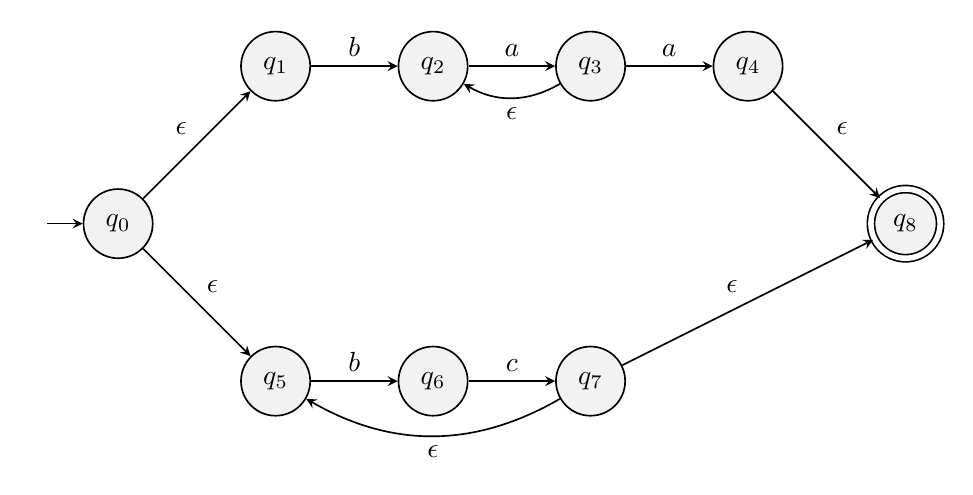
\begin{tikzpicture}
    \node[state, initial] at (0, 2) (q0){$q_0$};
    \node[state] at (2, 4) (q1){$q_1$};
    \node[state] at (4, 4) (q2){$q_2$};
    \node[state] at (6, 4) (q3){$q_3$};
    \node[state] at (8, 4) (q4){$q_4$};
    \node[state] at (2, 0) (q5){$q_5$};
    \node[state] at (4, 0) (q6){$q_6$};
    \node[state] at (6, 0) (q7){$q_7$};
    \node[state, accepting] at (10, 2) (q8){$q_8$};

    \draw

    (q0) edge node{$\epsilon$} (q1)
    (q0) edge node{$\epsilon$} (q5)

    (q1) edge node{$b$} (q2)
    (q2) edge node{$a$} (q3)
    (q3) edge[bend left] node{$\epsilon$} (q2)
    (q3) edge node{$a$} (q4)
    (q4) edge node{$\epsilon$} (q8)

    (q5) edge node{$b$} (q6)
    (q6) edge node{$c$} (q7)
    (q7) edge[bend left] node{$\epsilon$} (q5)
    (q7) edge node{$\epsilon$} (q8)

    ;
  \end{tikzpicture}

  \caption{Simplified $\epsilon$-NFA}
\end{figure}

and the table is

\begin{table}[H]
  \centering

  \begin{tabular}{c|cccc}
    state             & $\epsilon$               & a                    & b                    & c                    \\ \hline
    $\rightarrow q_0$ & $\left\{q_1,q_5\right\}$ & \O                   & \O                   & \O                   \\
    $q_1$             & \O                       & \O                   & $\left\{q_2\right\}$ & \O                   \\
    $q_2$             & \O                       & $\left\{q_3\right\}$ & \O                   & \O                   \\
    $q_3$             & $\left\{q_2\right\}$     & $\left\{q_4\right\}$ & \O                   & \O                   \\
    $q_4$             & $\left\{q_8\right\}$     & \O                   & \O                   & \O                   \\
    $q_5$             & \O                       & \O                   & $\left\{q_6\right\}$ & \O                   \\
    $q_6$             & \O                       & \O                   & \O                   & $\left\{q_7\right\}$ \\
    $q_7$             & $\left\{q_5,q_8\right\}$ & \O                   & \O                   & \O                   \\
    $* q_8$           & \O                       & \O                   & \O                   & \O
  \end{tabular}

  \caption{$\epsilon$-NFA Table}
\end{table}

\section{NFA}

First, we compute the $\epsilon$-closure table

\begin{table}[H]
  \centering

  \begin{tabular}{c|c}
    state             & $\epsilon$-closure           \\ \hline
    $\rightarrow q_0$ & $\left\{q_0,q_1,q_5\right\}$ \\
    $q_1$             & $\left\{q_1\right\}$         \\
    $q_2$             & $\left\{q_2\right\}$         \\
    $q_3$             & $\left\{q_2,q_3\right\}$     \\
    $* q_4$           & $\left\{q_4,q_8\right\}$     \\
    $q_5$             & $\left\{q_5\right\}$         \\
    $q_6$             & $\left\{q_6\right\}$         \\
    $* q_7$           & $\left\{q_5,q_7,q_8\right\}$ \\
    $* q_8$           & $\left\{q_8\right\}$
  \end{tabular}

  \caption{$\epsilon$-closure}
\end{table}

By lazy evaluation, we can compute the following NFA table

\begin{table}[H]
  \centering

  \begin{tabular}{c|ccc}
    state             & $a$                      & $b$                      & $c$                  \\ \hline
    $\rightarrow q_0$ & \O                       & $\left\{q_2,q_6\right\}$ & \O                   \\
    $q_1$             & \O                       & $\left\{q_2\right\}$     & \O                   \\
    $q_2$             & $\left\{q_3\right\}$     & \O                       & \O                   \\
    $q_3$             & $\left\{q_3,q_4\right\}$ & \O                       & \O                   \\
    $* q_4$           & \O                       & \O                       & \O                   \\
    $q_5$             & \O                       & $\left\{q_6\right\}$     & \O                   \\
    $q_6$             & \O                       & \O                       & $\left\{q_7\right\}$ \\
    $* q_7$           & \O                       & $\left\{q_6\right\}$     & \O                   \\
    $* q_8$           & \O                       & \O                       & \O
  \end{tabular}

  \caption{NFA Table}
\end{table}

Thus we can draw out the NFA

\begin{figure}[H]
  \centering

  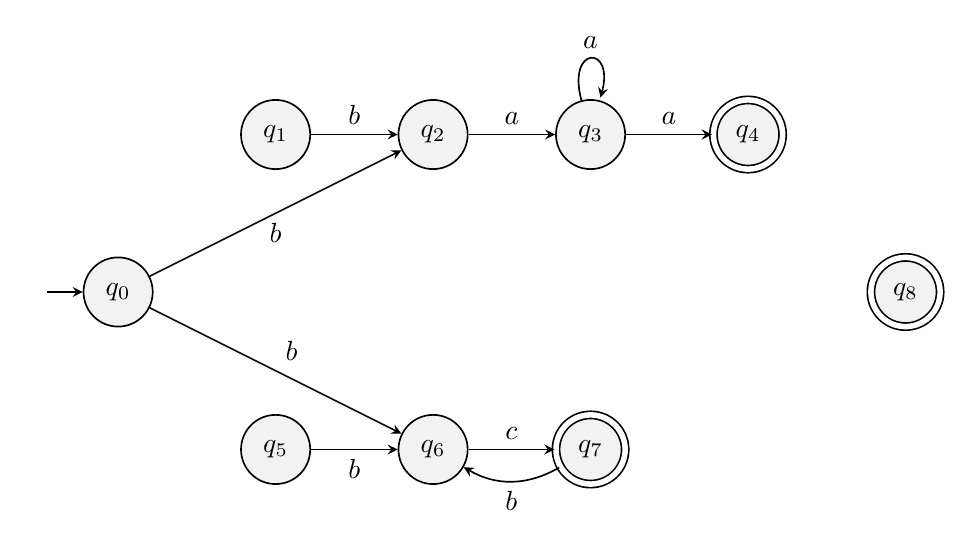
\begin{tikzpicture}
    \node[state, initial] at (0, 2) (q0){$q_0$};
    \node[state] at (2, 4) (q1){$q_1$};
    \node[state] at (4, 4) (q2){$q_2$};
    \node[state] at (6, 4) (q3){$q_3$};
    \node[state, accepting] at (8, 4) (q4){$q_4$};
    \node[state] at (2, 0) (q5){$q_5$};
    \node[state] at (4, 0) (q6){$q_6$};
    \node[state, accepting] at (6, 0) (q7){$q_7$};
    \node[state, accepting] at (10, 2) (q8){$q_8$};

    \draw

    (q0) edge[below] node{$b$} (q2)
    (q0) edge node{$b$} (q6)

    (q1) edge node{$b$} (q2)
    (q2) edge node{$a$} (q3)
    (q3) edge[loop above] node{$a$} (q3)
    (q3) edge node{$a$} (q4)

    (q5) edge[below] node{$b$} (q6)
    (q6) edge node{$c$} (q7)
    (q7) edge[bend left] node{$b$} (q6)

    ;
  \end{tikzpicture}

  \caption{NFA}
\end{figure}

We can safely remove $q_1$ and $q_5$ which are source vertices but not initial states as well as the independent state $q_8$. Thus the simplified NFA will be

\begin{figure}[H]
  \centering

  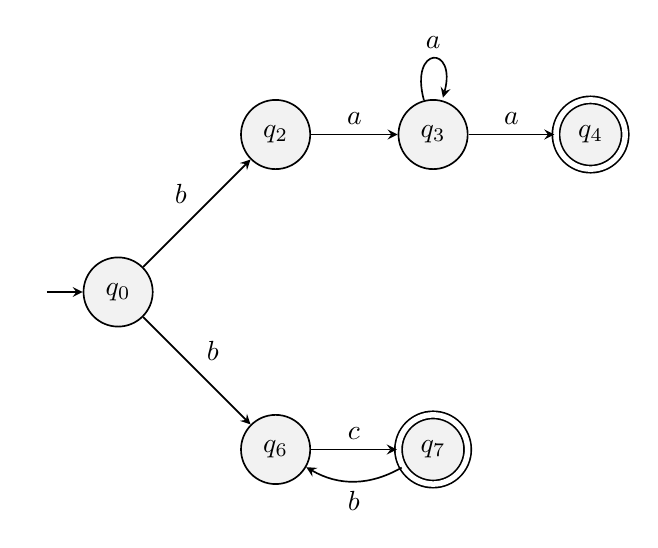
\begin{tikzpicture}
    \node[state, initial] at (0, 2) (q0){$q_0$};
    \node[state] at (2, 4) (q2){$q_2$};
    \node[state] at (4, 4) (q3){$q_3$};
    \node[state, accepting] at (6, 4) (q4){$q_4$};
    \node[state] at (2, 0) (q6){$q_6$};
    \node[state, accepting] at (4, 0) (q7){$q_7$};

    \draw

    (q0) edge node{$b$} (q2)
    (q0) edge node{$b$} (q6)

    (q2) edge node{$a$} (q3)
    (q3) edge[loop above] node{$a$} (q3)
    (q3) edge node{$a$} (q4)

    (q6) edge node{$c$} (q7)
    (q7) edge[bend left] node{$b$} (q6)

    ;
  \end{tikzpicture}

  \caption{Simplified NFA}
\end{figure}

\section{DFA}

The table for DFA converted from the NFA below is

\begin{table}[H]
  \centering

  \begin{tabular}{c|ccc}
    state                            & $a$                      & $b$                      & $c$                  \\ \hline
    $\rightarrow \left\{q_0\right\}$ & \O                       & $\left\{q_2,q_6\right\}$ & \O                   \\
    $\left\{q_2,q_6\right\}$         & $\left\{q_3\right\}$     & \O                       & $\left\{q_7\right\}$ \\
    $\left\{q_3\right\}$             & $\left\{q_3,q_4\right\}$ & \O                       & \O                   \\
    $* \left\{q_7\right\}$           & \O                       & $\left\{q_6\right\}$     & \O                   \\
    $* \left\{q_3,q_4\right\}$       & $\left\{q_3,q_4\right\}$ & \O                       & \O                   \\
    $\left\{q_6\right\}$             & \O                       & \O                       & $\left\{q_7\right\}$
  \end{tabular}

  \caption{DFA Table}
\end{table}

Thus the DFA is

\begin{figure}[H]
  \centering

  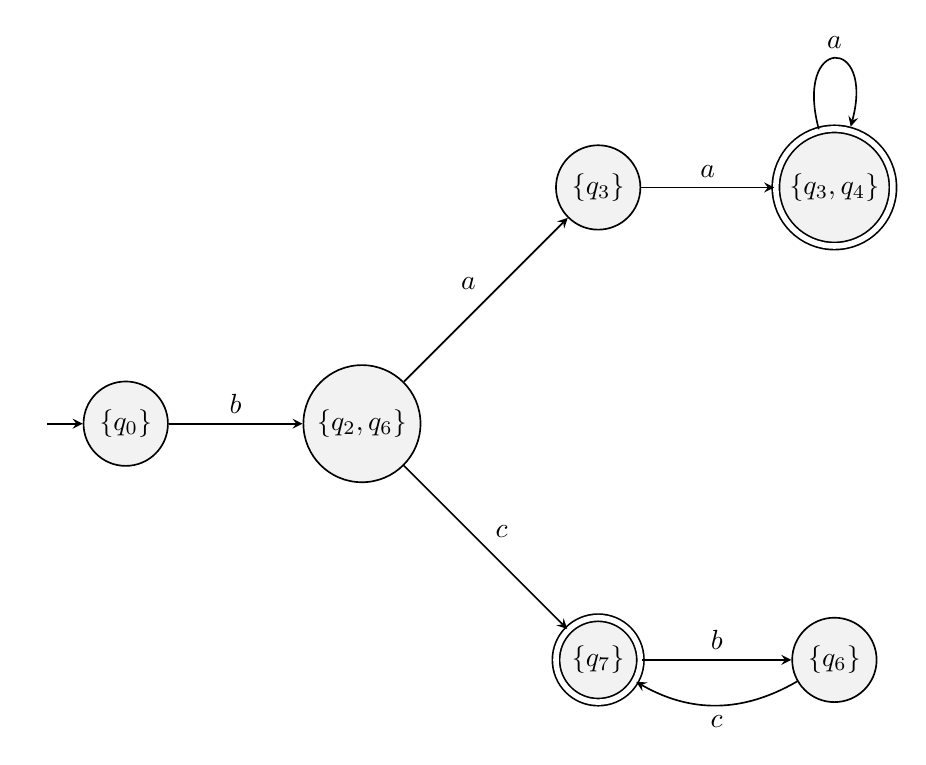
\begin{tikzpicture}
    \node[state, initial] at (0, 3) (q0){$\left\{q_0\right\}$};
    \node[state] at(3, 3) (q2_q6){$\left\{q_2,q_6\right\}$};
    \node[state] at (6, 6) (q3){$\left\{q_3\right\}$};
    \node[state, accepting] at (9, 6) (q3_q4){$\left\{q_3,q_4\right\}$};
    \node[state, accepting] at (6, 0) (q7){$\left\{q_7\right\}$};
    \node[state] at (9, 0) (q6){$\left\{q_6\right\}$};

    \draw

    (q0) edge node{$b$} (q2_q6)

    (q2_q6) edge node{$a$} (q3)
    (q3) edge node{$a$} (q3_q4)
    (q3_q4) edge[loop above] node {$a$} (q3_q4)

    (q2_q6) edge node{$c$} (q7)
    (q7) edge node{$b$} (q6)
    (q6) edge[bend left] node{$c$} (q7)

    ;
  \end{tikzpicture}

  \caption{DFA}
\end{figure}

which kind of rearrange and simplify the original RegEx.

\end{document}
